% Shared body of the submission (anonymous) and the preprint.
% Every number in the prose is a macro from tables/numbers.tex, written by bench/analyze.py.

\begin{abstract}
Multi-agent code verifiers split review into specialist agents (correctness, security, performance, style) and combine their verdicts, on the premise that specialists catch different defects. We test that premise on labels that come from running tests. The benchmark has 164 HumanEvalFix buggy/fixed function pairs and 300 SWE-bench Verified patches from two public agents, each labeled by the official harness, plus the 150 merged human fixes for the same tasks. CodeX-Verify, a four-agent rule-based verifier, is at chance: ROC-AUC \nHefCvAuc{} on HumanEvalFix, where it gives the buggy and the fixed function the same score in \nHefCvTie\% of pairs, and \nPaClaudeAuc{} and \nPaGptAuc{} on each agent's SWE-bench patches when it scores only the issues a patch introduces. Semgrep and Bandit are also at chance. A single LLM judge separates passing from failing SWE-bench patches (AUC \nSweSonnetAuc{} for Claude Sonnet 5.5, \nSweHaikuAuc{} for Haiku 5.5). Its reasons often cite the upstream fix, so absolute accuracy on this public benchmark partly reflects recall. Splitting the same judge into four role-prompted specialists does not measurably help under any aggregation (mean, max, weighted, vote, or a cross-validated logistic stack), and averaging three runs of the single judge beats the four-agent mean at lower cost. The specialists are redundant. Their verdicts add \nSonnetPermObs{} bits about the label beyond the correctness agent's, against \nSonnetPermNull{} bits expected if they were conditionally independent. We also re-examine the 99 self-labeled samples behind an earlier evaluation of CodeX-Verify: its \nOldCvAcc\% accuracy is below the \nOldMajority\% of always answering ``buggy'', and \nOldBugComments{} samples state their bug in a comment. We release the benchmark, every verifier output, and the analysis code.
\end{abstract}

\section{Introduction}

Coding agents now write patches faster than people can review them, so a cheap verifier that rejects wrong patches before tests or review would be valuable. A popular design is a team of specialist reviewer agents. Each agent checks one concern, and an aggregator combines their verdicts. The case for the team is the ensemble argument: members that err on different inputs combine into a better classifier \citep{dietterich2000ensemble}.

We test this design on labels that come from execution, and the answer is negative on both of its common forms. A rule-based four-agent verifier, CodeX-Verify, cannot tell correct code from incorrect code. A single LLM judge can, and giving the same model four specialist roles does not improve it. The two failures have different causes. The rule-based agents carry no information about functional correctness. The LLM specialists carry information, but the same information.

\paragraph{Contributions.}
\begin{itemize}
\item An execution-labeled verification benchmark of 778 items: 164 buggy/fixed function pairs from HumanEvalFix, re-verified by running the tests, and 450 SWE-bench Verified patches (300 from two public agents, labeled by the official harness, plus 150 merged human fixes) (\S\ref{sec:bench}).
\item A paired comparison of rule-based, static-analysis, and LLM verifiers on the same items, with ROC and precision--recall curves, cluster-bootstrap intervals, and compute-matched and stacked controls (\S\ref{sec:results}).
\item Measurements of the dependence assumption behind multi-agent verification: within-class rank correlations, conditional mutual information, and a permutation test of how much the specialists add beyond one agent (\S\ref{sec:dependence}).
\item A re-examination of an earlier evaluation of CodeX-Verify \citep{rajan2025codexverify}, which used 99 self-labeled samples (\S\ref{sec:v1}).
\end{itemize}

\section{Related Work}

\paragraph{Verifying LLM-generated code without execution.}
CodeJudge \citep{codejudge2024} asks an LLM to judge semantic correctness without test cases. CodeJudgeBench \citep{codejudgebench2025} evaluates 26 judges on generation, repair, and test-generation tasks and finds them sensitive to answer order. For repository-level patches, verifiers trained on agent trajectories rerank candidate SWE-bench patches \citep{swegym2024}. R2E-Gym \citep{r2egym2025} finds that execution-free verifiers lean on stylistic features and gain most when combined with execution-based ones. Agentic Rubrics \citep{agenticrubrics2026} scores patches against a repository-specific rubric written by an agent, and Dockerless \citep{dockerless2026} builds an agentic patch verifier that needs no execution environment. These systems are rerankers built on one verifier. We hold the model fixed and ask whether splitting it into specialists helps.

\paragraph{Multi-agent judges.}
ChatEval \citep{chan2023chateval} reports that diverse personas help multi-agent debate evaluate open-ended text, and Agent-as-a-Judge \citep{zhuge2024agentasjudge} uses an agentic judge to evaluate code-generating agents. CodeAgent \citep{tang2024codeagent} coordinates role-specialized agents for code review. Against these, several controlled studies find that multi-agent gains shrink under matched compute. Single agents match multi-agent systems on multi-hop reasoning at equal thinking budgets, explained by a data-processing-inequality argument \citep{trankiela2026}. Automatically designed multi-agent systems underperform chain-of-thought with self-consistency at up to ten times the cost \citep{jwalapuram2026illusion}. Majority voting explains most of the gain of multi-agent debate \citep{choi2025debate}. Self-correction without external feedback is limited \citep{huang2024selfcorrect,kamoi2024selfcorrect,stechly2024selfverify}, and LLM judges carry self-preference and other biases \citep{wataoka2024selfpref,ye2024justice}. Ensemble theory states the condition directly: members must be both accurate and diverse \citep{dietterich2000ensemble,kuncheva2003diversity}. We measure both properties for verifier agents.

\paragraph{Label quality in code benchmarks.}
Passing SWE-bench tests does not guarantee a correct patch. PatchDiff \citep{patchdiff2025} and UTBoost \citep{utboost2025} find patches that pass the official tests and behave differently from the reference fix. SWEPatchTest \citep{swepatchtest2026} shows that generated tests rarely separate correct from incorrect patches. SWEADV \citep{sweadv2026} reports 39.4\% detection accuracy for static analysis and 55.4\% for an LLM judge on adversarial security patches. PrimeVul \citep{primevul2024} shows that vulnerability detectors drop sharply on paired data, where a vulnerable function and its patched version must be told apart; our HumanEvalFix pairs apply the same discipline to functional bugs.

\paragraph{Relationship to the earlier CodeX-Verify evaluation.}
\citet{rajan2025codexverify} introduced CodeX-Verify and reported \nOldCvTpr\% TPR and \nOldCvAcc\% accuracy on 99 samples, a 15-subset ablation, and an information-theoretic argument for combining agents. We evaluate the same system on execution-labeled data, add the baselines that evaluation lacked, and replace its theory with measured dependence. Section~\ref{sec:v1} reports what its 99-sample set measured.

\section{Benchmark}
\label{sec:bench}

\paragraph{HumanEvalFix pairs.}
HumanEvalFix \citep{muennighoff2024octopack} injects one human-written bug into each of the 164 HumanEval solutions \citep{chen2021humaneval}. Each item is the HumanEval prompt (signature and docstring) followed by either the canonical body (correct) or the buggy body (incorrect). We ran every item against the HumanEval tests: all 164 canonical versions pass and all 164 buggy versions fail. The two versions differ only in the bug, so any verifier signal that ignores the bug cancels within a pair. No item names its bug; one function carries the comment ``remove trailing zeros'' in both versions.

\paragraph{SWE-bench Verified patches.}
We sampled 150 SWE-bench Verified tasks \citep{jimenez2024swebench,openai2024sweverified} (seed 0) for which two public leaderboard submissions both produced a non-empty patch: Claude 3.5 Sonnet with Anthropic's tools scaffold (20241022) and Agentless 1.5 with GPT-4o (20241028). A patch is incorrect when the official harness marks it unresolved, which holds for 161 of the 300. We add the 150 merged human fixes for the same tasks, all correct. For tools that need whole files, we fetch each touched Python file at the task's base commit and apply the patch. Main SWE-bench results use the 300 agent patches; for gold patches we report how often each verifier rejects a known-correct fix.

\paragraph{Label quality and contamination.}
All labels come from executing tests. They are imperfect: SWE-bench tests accept some wrong patches \citep{patchdiff2025,utboost2025}, and HumanEval tests are short. Both benchmarks are public and old enough to be in LLM training data, and Section~\ref{sec:results} measures how often the LLM judges cite the reference fix.

\section{Verifiers}
\label{sec:verifiers}

Every verifier scores the same items and returns a continuous score (for ROC/PR) and a binary flag (for an operating point).

\paragraph{CodeX-Verify.}
Four rule-based agents analyze the code. Correctness checks AST complexity, nesting, exception coverage, input validation, and edge-case guards; it also runs the code as a script when the code contains none of a list of dangerous patterns, and raises a HIGH issue if the run fails. Security matches 15+ CWE patterns and secret regexes. Performance estimates loop and recursion complexity. Style computes maintainability and documentation metrics. The aggregator combines agent scores with fixed weights (security 0.45, correctness 0.35, performance 0.15, style 0.05), applies severity caps, and returns PASS, WARNING, or FAIL. The score is one minus the system's overall score; the flag is ``not PASS'', and Table~\ref{tab:main} also reports FAIL-only. The 15 agent subsets pass the corresponding agent results to the same aggregator. On SWE-bench we run two input modes. \emph{Snippet} mode, used by the earlier evaluation, analyzes the added and context lines of the diff. \emph{Patch-aware} mode runs the agents on each touched file before and after the patch and scores the severity-weighted issues the patch introduces.

\paragraph{Static analyzers.}
Semgrep \citep{semgrep} with the \texttt{p/python}, \texttt{p/security-audit}, \texttt{p/default}, \texttt{p/r2c-best-practices}, and \texttt{p/r2c-bug-scan} packs, and Bandit \citep{bandit}. On SWE-bench both count findings the patch introduces.

\paragraph{LLM verifiers.}
The \emph{single judge} receives the function, or the issue text and the patch, and returns, as structured JSON, a probability (0--100) that the code should be rejected and an ACCEPT/REJECT verdict. The \emph{four-agent} verifier makes four calls with the same model and input, each told to focus only on correctness, security, performance, or style, mirroring CodeX-Verify's roles. We combine their probabilities by mean, max, CodeX-Verify's weights, and a logistic stack fit with 5-fold cross-validation grouped by task, and their verdicts by majority (3 of 4) and any-reject. As a compute-matched control, we average three independent runs of the single judge. We use Claude Sonnet 5.5 and Claude Haiku 5.5 at low reasoning effort; patches over 30,000 characters are truncated (\nNTruncated{} of 450). Prompts are in Appendix~\ref{app:prompts}.

\paragraph{Trivial baselines.}
\emph{Always flag}; a \emph{majority vote} of CodeX-Verify's agents, each run through the aggregator alone; and, on SWE-bench, single patch features (length, changed lines, files touched, which agent wrote it).

\paragraph{Metrics.}
ROC-AUC and average precision from the score; TPR, FPR, and balanced accuracy at the flag. Intervals are 95\% percentile intervals from 2,000 bootstrap resamples of clusters (a HumanEvalFix pair; a SWE-bench task, which carries two agent patches). Verifier differences use paired bootstrap on the same resamples \citep{efron1994bootstrap}, with Holm correction across the \nHolmN{} single-judge versus specialist comparisons.

\section{Results}
\label{sec:results}

\begin{table*}[t]
\centering
\footnotesize
\begin{tabular}{@{}l ccc ccc c@{}}
\toprule
 & \multicolumn{3}{c}{HumanEvalFix (164 buggy / 164 fixed)} & \multicolumn{3}{c}{SWE-bench Verified agent patches} & Gold \\
\cmidrule(lr){2-4}\cmidrule(lr){5-7}
Verifier & AUC [95\% CI] & TPR & FPR & AUC [95\% CI] & TPR & FPR & flagged \\
\midrule
Always flag & 0.50 [0.50, 0.50] & 100.0 & 100.0 & 0.50 [0.50, 0.50] & 100.0 & 100.0 & 100.0 \\
\midrule
CodeX-Verify (FAIL) & 0.50 [0.49, 0.52] & 17.7 & 17.7 & 0.48 [0.47, 0.50] & 98.1 & 99.3 & 99.3 \\
CodeX-Verify (FAIL or WARN) & 0.50 [0.49, 0.52] & 78.7 & 78.7 & 0.48 [0.47, 0.50] & 99.4 & 100.0 & 100.0 \\
Static agents, majority vote & 0.50 [0.49, 0.51] & 1.8 & 1.8 & 0.51 [0.47, 0.55] & 15.5 & 12.2 & 10.7 \\
CodeX-Verify, patch-aware & \multicolumn{3}{c}{n/a} & 0.47 [0.42, 0.53] & 55.3 & 55.4 & 26.7 \\
\midrule
Semgrep & 0.50 [0.50, 0.51] & 2.4 & 1.8 & 0.52 [0.49, 0.55] & 8.7 & 5.0 & 2.0 \\
Bandit & 0.50 [0.50, 0.50] & 1.8 & 1.8 & 0.48 [0.44, 0.52] & 11.2 & 15.1 & 2.0 \\
\midrule
Haiku 5.5 single judge & 0.99 [0.98, 1.00] & 98.8 & 11.6 & 0.83 [0.78, 0.88] & 81.4 & 30.9 & 13.3 \\
Haiku 5.5 4 agents, mean & 0.98 [0.96, 0.99] & 36.6 & 1.8 & 0.79 [0.73, 0.85] & 36.0 & 10.8 & 1.3 \\
Haiku 5.5 4 agents, majority vote & 0.98 [0.96, 0.99] & 34.1 & 1.2 & 0.78 [0.72, 0.84] & 36.0 & 12.2 & 2.7 \\
Sonnet 5.5 single judge & 1.00 [0.99, 1.00] & 99.4 & 3.0 & 0.89 [0.85, 0.93] & 85.1 & 20.9 & 4.7 \\
Sonnet 5.5 correctness agent & 1.00 [1.00, 1.00] & 100.0 & 5.5 & 0.91 [0.87, 0.94] & 84.5 & 18.0 & 4.7 \\
Sonnet 5.5 4 agents, mean & 0.99 [0.98, 1.00] & 82.9 & 1.8 & 0.88 [0.83, 0.92] & 72.7 & 14.4 & 1.3 \\
Sonnet 5.5 4 agents, max & 1.00 [1.00, 1.00] & 100.0 & 11.0 & 0.86 [0.81, 0.90] & 91.9 & 56.1 & 5.3 \\
Sonnet 5.5 4 agents, weighted & 0.99 [0.98, 1.00] & 57.9 & 0.6 & 0.89 [0.85, 0.93] & 64.6 & 6.5 & 1.3 \\
Sonnet 5.5 4 agents, majority vote & 0.99 [0.98, 1.00] & 64.6 & 1.8 & 0.87 [0.83, 0.92] & 72.7 & 14.4 & 1.3 \\
Sonnet 5.5 4 agents, any reject & 0.99 [0.98, 1.00] & 100.0 & 13.4 & 0.87 [0.83, 0.92] & 92.5 & 58.3 & 5.3 \\
\bottomrule
\end{tabular}

\caption{Verifiers on the same execution-labeled items. AUC with 95\% cluster-bootstrap CI; TPR and FPR (\%) at each verifier's flag. ``Gold flagged'' is the share of the 150 merged human fixes the verifier rejects (all are correct). CodeX-Verify on SWE-bench uses snippet mode unless marked patch-aware.}
\label{tab:main}
\end{table*}

\begin{figure*}[t]
\centering
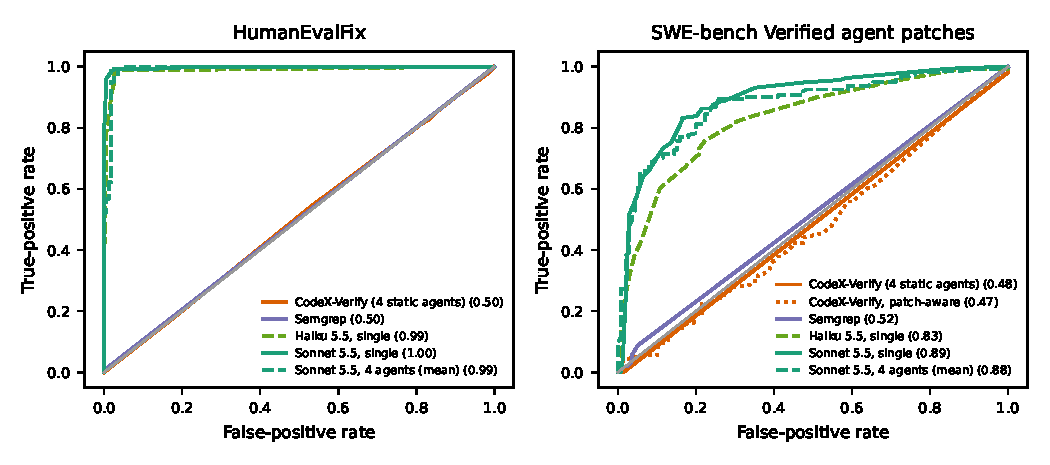
\includegraphics[width=0.85\textwidth]{figures/roc.pdf}
\caption{ROC curves (AUC in parentheses). The rule-based and static verifiers lie on the diagonal on both benchmarks; the LLM judges do not.}
\label{fig:roc}
\end{figure*}

\subsection{The rule-based multi-agent verifier is at chance}

Table~\ref{tab:main} and Figure~\ref{fig:roc} give the main result. On HumanEvalFix, CodeX-Verify's AUC is \nHefCvAuc{} [\nHefCvAucLo, \nHefCvAucHi], its TPR equals its FPR (\nHefCvTpr\%), and it scores the buggy and fixed versions of a function identically in \nHefCvTie\% of pairs. Its most frequent HIGH finding, \texttt{potential\_bug}, fires on \nHefPotentialBugBuggy\% of buggy and \nHefPotentialBugFixed\% of fixed functions. Each agent alone has AUC between \nHefAgentAucMin{} and \nHefAgentAucMax.

On SWE-bench, the patch-aware mode has AUC \nPaClaudeAuc{} on the Claude agent's patches and \nPaGptAuc{} on Agentless's. Pooled over both agents it is \nSweCvDiffAuc{}, lower than either because the Claude agent leaves helper scripts in its patches, which raises its mean score (\nPaClaudeScore{} against \nPaGptScore) independently of the label. For calibration, the length of a patch alone has AUC \nTrivLen, its number of changed lines \nTrivLines, and the identity of the agent that wrote it \nTrivGen.

Snippet mode, the input the earlier evaluation used, rejects almost everything: \nSweCvTpr\% of failing patches, \nSweCvFpr\% of passing ones, and \nGoldCv\% of human fixes. The snippet is not valid Python in \nSweSyntaxCrit{} of \nSweNItems{} patches, and the Correctness agent turns the parse error into a CRITICAL issue that forces FAIL. The same agent executes the snippet and raises a HIGH issue for the \nSweExecHigh{} that crash. The earlier evaluation's report that 99\% of 300 SWE-bench patches fail comes from this effect: it ran on SWE-bench Lite's gold fixes, and \nLiteSyntax{} of its \nLiteN{} snippets carry the same CRITICAL parse issue.

Semgrep and Bandit stay silent on most inputs and have AUC \nSweSemgrepAuc{} and \nSweBanditAuc{} on SWE-bench. Both benchmarks contain functional bugs, which their rule packs do not target.

\subsection{A single LLM judge separates passing from failing patches, partly by recall}

A single Sonnet 5.5 judge has AUC \nHefSonnetAuc{} on HumanEvalFix, ranking the buggy version above the fixed one in \nHefSonnetPairWin\% of pairs. On SWE-bench its AUC is \nSweSonnetAuc{} [\nSweSonnetAucLo, \nSweSonnetAucHi], with TPR \nSweSonnetTpr\% at FPR \nSweSonnetFpr\%, and it rejects \nGoldSonnet\% of human fixes. Across \nSonnetRuns{} runs its AUC is \nSonnetRunMean{} $\pm$ \nSonnetRunSd. Haiku 5.5, at a twentieth of the price per token, reaches \nSweHaikuAuc.

The judge sees only the issue and the diff, yet Sonnet's reasons cite an upstream or reference fix for \nSonnetRecallAgent\% of agent patches and \nSonnetRecallGold\% of gold patches; Haiku's do for \nHaikuRecallAgent\% and \nHaikuRecallGold\%. On SWE-bench Verified the judge often compares the patch with a fix it remembers, so its absolute accuracy overstates what it would achieve on unseen code. The discrimination does not come from the mentions: on the patches where Haiku cites no reference fix (\nHaikuCleanN{} of 300) its AUC is \nHaikuCleanAuc, against \nHaikuMentionedAuc{} where it does. The judge is also no better on patches from a Claude model (AUC \nGenClaudeSonnetAuc) than on GPT-4o's (\nGenGptSonnetAuc; Appendix Table~\ref{tab:generators}).

\subsection{Role-prompted specialists do not improve the LLM judge}

Holding the model fixed, we compare the single judge with the four-agent verifier built from the same model (Table~\ref{tab:main}, lower block). On SWE-bench, Sonnet's four-agent AUC is \nSweSonnetMeanAuc{} (mean), \nSweSonnetWeightedAuc{} (weighted), \nSweSonnetMaxAuc{} (max), and \nSonnetStackAuc{} (cross-validated logistic stack), against \nSonnetSingleAucExact{} for the single judge. The paired difference for the mean is \nSweDiffSonnetSingleJudgeVsSonnetAgentsMean{} [\nSweDiffSonnetSingleJudgeVsSonnetAgentsMeanLo, \nSweDiffSonnetSingleJudgeVsSonnetAgentsMeanHi] in favor of the single judge, which rules out a gain from the specialists larger than \nSweDiffSonnetSingleJudgeVsSonnetAgentsMeanLoAbs{} AUC at this sample size. With Haiku the stack reaches \nHaikuStackAuc{} against \nHaikuSingleAucExact{} for the single judge. Averaging three runs of the single judge, which costs three calls to the specialists' four, reaches \nSweSonnetThreeAuc, \nSweDiffSonnetSingleJudgeMeanOfRunsVsSonnetAgentsMean{} [\nSweDiffSonnetSingleJudgeMeanOfRunsVsSonnetAgentsMeanLo, \nSweDiffSonnetSingleJudgeMeanOfRunsVsSonnetAgentsMeanHi] above the four-agent mean. After Holm correction no single comparison is significant (smallest adjusted $p$ = \nHolmMinP), so the evidence is that specialists add nothing measurable, not that they hurt. Verdict-level rules move the operating point without improving the trade-off: any-reject raises Sonnet's TPR to \nSweSonnetAnyRejectTpr\% at an FPR of \nSweSonnetAnyRejectFpr\%, and the mean rule lowers both (\nSweSonnetMeanTpr\% and \nSweSonnetMeanFpr\%).

The recall effect does not explain this result. On the \nHaikuCleanAllN{} patches where none of Haiku's five calls cites a reference fix, the single judge has AUC \nHaikuCleanAllSingleAuc{} and the four-agent mean \nHaikuCleanAllMeanAuc.

The best LLM verifier is the correctness agent alone (AUC \nSweSonnetCorrAuc{} with Sonnet, \nSweHaikuCorrAuc{} with Haiku), which is one judge with a narrower prompt; its difference from the generalist is within noise (\nSweDiffSonnetSingleJudgeVsSonnetCorrectnessAgent{} [\nSweDiffSonnetSingleJudgeVsSonnetCorrectnessAgentLo, \nSweDiffSonnetSingleJudgeVsSonnetCorrectnessAgentHi]). Our labels measure functional correctness only, so the security, performance, and style agents could help only by noticing functional bugs; they do notice them, as the next section shows, and so add no new information.

\subsection{The rule-based ablation attributes nothing}

The earlier evaluation's 15-subset ablation attributed most of the detection to the Correctness agent. On execution labels every subset is at chance, with AUC from \nHefAblWorst{} to \nHefAblBest{} on HumanEvalFix and \nSweAblWorst{} to \nSweAblBest{} on SWE-bench (Appendix Table~\ref{tab:ablation}). The agents' Shapley values for AUC are all within $\pm0.03$.

\section{Measured Agent Dependence}
\label{sec:dependence}

Write $B$ for the label and $A_S$ for the outputs of an agent set $S$. By the chain rule, $I(A_{S\cup\{i\}};B)=I(A_S;B)+I(A_i;B\mid A_S)$, and the last term is non-negative \citep{cover2006elements}, so adding an agent never lowers the information in the agents' joint output. This fact constrains little. A fixed aggregator $\psi$ can discard information, since $I(\psi(A_S);B)\le I(A_S;B)$; the gain is zero for an agent whose information is already in $A_S$; and $S\mapsto I(A_S;B)$ is submodular, so that additions show diminishing returns and greedy selection is near-optimal \citep{nemhauser1978analysis}, only when the agents are conditionally independent given $B$ \citep{krause2005nearoptimal}. The earlier evaluation assumed that independence. We measure it.

\begin{table*}[t]
\centering
\footnotesize
\begin{tabular}{@{}l cccc@{}}
\toprule
Agent pair & Static, HEF & Static, SWE & LLM, HEF & LLM, SWE \\
\midrule
C-S & 0.06 / 0.06 & 0.07 / 0.09 & 0.47 / 0.24 & 0.62 / 0.66 \\
C-P & -0.08 / -0.10 & -0.26 / -- & 0.35 / 0.52 & 0.80 / 0.89 \\
C-St & 0.17 / 0.18 & 0.20 / 0.10 & 0.50 / 0.73 & 0.63 / 0.79 \\
S-P & -0.03 / -0.02 & -0.04 / -- & 0.56 / 0.42 & 0.69 / 0.69 \\
S-St & 0.13 / 0.12 & 0.06 / 0.13 & 0.49 / 0.32 & 0.73 / 0.70 \\
P-St & 0.17 / 0.17 & -0.08 / -- & 0.58 / 0.56 & 0.75 / 0.86 \\
\midrule
$\hat I(D_{C};B)$ (bits) & 0.000 & 0.006 & 0.844 & 0.347 \\
$\hat I(D_{C+S};B)$ (bits) & 0.000 & 0.009 & 0.846 & 0.369 \\
$\hat I(D_{C+S+P};B)$ (bits) & 0.000 & 0.016 & 0.853 & 0.373 \\
$\hat I(D_{C+S+P+St};B)$ (bits) & 0.000 & 0.019 & 0.874 & 0.377 \\
\bottomrule
\end{tabular}

\caption{Agent dependence. Top: Spearman correlation between two agents' scores within correct / within incorrect items. Bottom: plug-in mutual information (bits) between the agents' binary verdicts and the label, for nested agent sets. Rule-based agents: CodeX-Verify (patch-aware on SWE-bench); LLM agents: Sonnet 5.5. HEF: HumanEvalFix; SWE: agent patches.}
\label{tab:corr}
\end{table*}

\paragraph{Rule-based agents.}
On HumanEvalFix the agents' within-class correlations are small (Table~\ref{tab:corr}) and their verdicts carry \nStaticHefMiAll{} bits about the label. In patch-aware mode on SWE-bench, their correlations range from \nPaRhoMin{} to \nPaRhoMax{}, because larger patches raise every agent's issue count, and each agent alone has AUC between \nPaAgentAucMin{} and \nPaAgentAucMax. The rule-based agents fail the first condition of the ensemble argument: none is informative, so combining them cannot help.

\paragraph{LLM agents.}
Each LLM agent is informative (the correctness agent's verdict carries \nSonnetSweMiC{} bits on SWE-bench), but within each class their scores correlate at $\rho$ = \nSonnetSweRhoMin--\nSonnetSweRhoMax, and the four verdicts together carry \nSonnetSweMiAll{} bits. To test whether this redundancy exceeds chance, we shuffle the security, performance, and style verdicts within each class, which keeps each agent's class-conditional rates and removes its dependence on the correctness agent. Under that null the three would add \nSonnetPermNull{} bits beyond the correctness agent (5th percentile \nSonnetPermNullLo); they add \nSonnetPermObs{} (\nSonnetPermObsMm{} with the Miller--Madow correction). For Haiku the figures are \nHaikuPermNull{} expected and \nHaikuPermObs{} observed. The agents also ignore their roles. On HumanEvalFix the style agent's verdict carries \nSonnetHefMiSt{} bits about functional bugs, close to the correctness agent's \nSonnetHefMiC: a model asked to judge style still notices when the function is wrong. The LLM agents fail the second condition: they are accurate and redundant.

\section{The Earlier 99-Sample Evaluation}
\label{sec:v1}

We reconstructed the 99 samples of the earlier evaluation from its released scripts: 29 hand-written samples and 70 that Claude generated together with their labels. Re-running the system on them reproduces the reported \nOldCvAcc\% accuracy, \nOldCvTpr\% TPR, and \nOldCvFpr\% FPR, counting FAIL as a rejection. The set is \nOldBuggy/\nOldN{} buggy, so always answering ``buggy'' scores \nOldMajority\%. \nOldBugComments{} samples contain a literal \texttt{\# BUG} comment, \nOldBugCommentsBuggy{} of them buggy. CodeX-Verify does not use these comments (\nOldCvStripAcc\% accuracy with comments removed). An LLM judge does: Sonnet 5.5 scores \nOldSonnetAcc\% with them and \nOldSonnetStripAcc\% without, and its TPR falls from \nOldSonnetTpr\% to \nOldSonnetStripTpr\%. Appendix Table~\ref{tab:claims} sets each claim of the earlier evaluation against the execution-labeled results. Two concern the system itself: it was described as static with no test execution, and its Correctness agent runs the code under analysis.

\section{Limitations}

The SWE-bench sample covers 150 tasks and two agents, and its labels come from tests that accept some incorrect patches. Both benchmarks are public, and the LLM judges recall reference fixes; the single-versus-specialist comparison holds on patches where no recall is cited, but absolute judge accuracy on unseen code is likely lower. The labels measure functional correctness only, so this study cannot show whether specialists help on security or performance defects. The LLM verifiers use one model family, one prompt per role, and low reasoning effort. All verifiers see the patch without the rest of the repository.

\section{Conclusion}

On execution-labeled code, a four-agent rule-based verifier and two standard static analyzers are at chance. A single LLM judge separates passing from failing SWE-bench patches, and role-prompted specialists built on the same model add nothing measurable, because they detect the same defects. Multi-agent verifiers should be evaluated on paired, execution-labeled data against a single-judge baseline at matched cost, and should report how much information each added agent contributes beyond the others.
